%%%%%%%%%%%%%%%%%%%%%%%%%%%%%%%%%%%%%%%%%
% Classic Lined Title Page
% LaTeX Template
% Version 1.0 (27/12/12)
%
% This template has been downloaded from:
% http://www.LaTeXTemplates.com
%
% Original author:
% Peter Wilson (herries.press@earthlink.net)
%
% License:
% CC BY-NC-SA 3.0 (http://creativecommons.org/licenses/by-nc-sa/3.0/)
%
% Instructions for using this template:
% This title page compiles as is. If you wish to include this title page in
% another document, you will need to copy everything before
% \begin{document} into the preamble of your document. The title page is
% then included using \titleAT within your document.
%
%%%%%%%%%%%%%%%%%%%%%%%%%%%%%%%%%%%%%%%%%

%----------------------------------------------------------------------------------------
%	PACKAGES AND OTHER DOCUMENT CONFIGURATIONS
%----------------------------------------------------------------------------------------



\documentclass[a4paper]{article}

\usepackage[utf8]{inputenc}
\usepackage{hyperref}
\usepackage{titlesec}
\usepackage{amssymb,amsmath}
\usepackage[italian]{babel}
\usepackage[titles]{tocloft}
\usepackage{appendix}
\hypersetup{%
    pdfborder = {0 0 0}
}
\usepackage{graphicx}
\usepackage[svgnames]{xcolor} % Required to specify font color
\usepackage{eurosym}

\newcommand*{\plogo}{\fbox{$\mathcal{PL}$}} % Generic publisher logo
\usepackage{listings}
\usepackage{fancyhdr}
\usepackage{lastpage}
\usepackage{ragged2e}
\usepackage{listingsutf8}
\usepackage{mathtools}\usepackage{chngcntr}
\usepackage{float}
\usepackage{longtable}

%----------------------------------------------------------------------------------------
%	TITLE PAGE
%----------------------------------------------------------------------------------------

\newcommand*{\titleAT}{\begingroup % Create the command for including the title page in the document
\newlength{\drop} % Command for generating a specific amount of whitespace
\drop=0.1\textheight % Define the command as 10% of the total text height

\rule{\textwidth}{1pt}\par % Thick horizontal line
\vspace{2pt}\vspace{-\baselineskip} % Whitespace between lines
\rule{\textwidth}{0.4pt}\par % Thin horizontal line

\vspace{\drop} % Whitespace between the top lines and title
\begin{center} % Center all text
\textcolor{Black}{ % Red font color
{\Huge Progetto}\\[0.5\baselineskip] % Title line 1
{\Large di}\\[0.75\baselineskip] % Title line 2
{\Huge Tecnologie Web 2}} % Title line 3
\\[2\baselineskip]
{\Large Analisi di usabilità di un sito web}

\vspace{0.25\drop} % Whitespace between the title and short horizontal line
\rule{1\textwidth}{0.4pt}\par % Short horizontal line under the title
\vspace{\drop} % Whitespace between the thin horizontal line and the author name

\begin{tabular}{l | r}

\hline
\textbf{Versione} & 1.0.0 \\
\hline
\textbf{Sito web analizzato} & html.it \\
\hline
\textbf{URL} & http://www.html.it \\
\hline
\textbf{Autore} & Luca De Franceschi \\
\hline
\textbf{Distribuzione} & Prof. Massimo Marchiori \\
\hline
\textbf{Periodo di analisi} & Giugno/Luglio 2014 \\
\hline

\end{tabular}

\end{center}

\vfill % Whitespace between the author name and publisher text
\vfill
{\large Università degli studi di Padova}



%\rule{\textwidth}{0.4pt}\par % Thin horizontal line
%\vspace{2pt}\vspace{-\baselineskip} % Whitespace between lines
%\rule{\textwidth}{1pt}\par % Thick horizontal line

\endgroup}

\titleformat{\chapter}[display]
{}{\hfill\rule{.7\textwidth}{3pt}}{2pt}
{\hspace*{.3\textwidth}\huge\bfseries}[\addvspace{1pt}]
\titleformat{name=\chapter,numberless}[display]
{}{\hfill\rule{.7\textwidth}{3pt}}{2pt}
{\hspace*{.3\textwidth}\huge\bfseries}[\addvspace{1pt}]

\renewcommand*\contentsname{Indice}

\newcommand{\glossario}[1]{\textit{#1\ped{G}}}

\lstset{frame=shadowbox,
  language=c++,
  aboveskip=10mm,
  belowskip=10mm,
  showstringspaces=false,
  columns=flexible,
  basicstyle={\small\ttfamily},
  numbers=none,
  numberstyle=\tiny\color{gray},
  keywordstyle=\color{blue},
  commentstyle=\color{gray},
  stringstyle=\color{red},
  breaklines=true,
  breakatwhitespace=true
  tabsize=1
}
\lstset{inputencoding=utf8/latin1}

\renewcommand{\lstlistingname}{Listato}
\renewcommand{\footrulewidth}{0.4pt}

\newcommand{\changefont}{%
    \fontsize{5}{7}\selectfont
}

\def\arraystretch{2}

\DeclarePairedDelimiter\ceil{\lceil}{\rceil}
\DeclarePairedDelimiter\floor{\lfloor}{\rfloor}

%----------------------------------------------------------------------------------------
%	CONSTANTS
%----------------------------------------------------------------------------------------

\newcommand{\authorName}{Luca De Franceschi}

%----------------------------------------------------------------------------------------
%	DOCUMENT HEADER
%----------------------------------------------------------------------------------------

\begin{document}
\titleAT % This command includes the title page
\pagestyle{empty}
\newpage
\tableofcontents
\newpage
\listoffigures
\clearpage

%----------------------------------------------------------------------------------------
%	HEADER FORMAT
%----------------------------------------------------------------------------------------

\fancyhf{}
\fancyhead[RE]{\small\scshape\nouppercase{\leftmark}}
\fancyhead[LO]{\small\scshape\nouppercase{\rightmark}}
\fancyhead[LE,RO]{\small\thepage}
\lhead{\rightmark}
\rhead{Progetto di Tecnologie web 2}
\rfoot{\thepage/\pageref{LastPage}}
\lfoot{\authorName}




%----------------------------------------------------------------------------------------
%	CONTENT
%----------------------------------------------------------------------------------------

\raggedright

\section*{Prefazione}

Risulta evidente come nell'ultimo decennio i metodi reperimento dell'informazione abbiano subito un cambiamento radicale. Oggigiorno reperire informazioni, conoscenza e quant'altro dal web rappresenta una \textit{condicio sine qua non}. Parlare di questo fenomeno risulterebbe noioso, in quanto è un tema scontato e già ampiamente discusso e documentato. La tecnologia non solo ci accompagna quotidianamente, ma è diventata parte integrante di noi stessi e del nostro modo di vivere; uno stile di vita in continua evoluzione, nel quale il rapporto uomo-macchina è sempre più stretto, basti immaginare alla percentuale di tempo che passiamo in compagnia del nostro smartphone o del nostro tablet.
\linebreak
\linebreak
Chiunque oggigiorno dovrebbe avere il sacrosanto diritto di \textbf{avere l'informazione a portata di mano} ed ottenere ciò che cerca \textbf{nel modo più facile e intuitivo possibile}. Il web è stato sviluppato esattamente con questo intento, anche se nella realtà attuale reperire informazioni è solamente una delle tante tipologie di richieste da parte degli utenti. In questa relazione ci occuperemo solamente del primo aspetto. Questo tema sembrerebbe a prima vista banale e poco interessante, ma se ci fermiamo per un'istante e pensiamo a quanti siti web nei quali navighiamo ogni giorno soddisfano realmente queste due necessità credo che dovremmo fare una bella scrematura.
\linebreak
\linebreak
Il web è in continua evoluzione. Un sito web sviluppato oggi in poco tempo diviene obsoleto, perchè cambiano i canoni di progettazione, che sono strettamente correlati alle crescenti e mutabili necessità degli utenti. E queste necessità sono sempre maggiori: gli utenti sono impazienti, vogliono pagine che si caricano velocemente, ben indicizzate dai motori di ricerca e, soprattuto, vogliono \textbf{trovare quel che cercano} in modo rapido. Se la pagina non riesce a soddisfare questo l'utente si dirigerà altrove. Ecco che in quest'ottica è necessario introdurre il termine \textbf{usabilità}, che viene definita come segue:

\begin{center}

\textit{``Il grado in cui un prodotto può essere usato da particolari utenti per raggiungere certi obiettivi con efficacia, efficienza, soddisfazione in uno specifico contesto d’uso''}\footnote{Definizione secondo ISO 9241-11:1998}

\end{center} 

Il contesto d'uso della presente relazione è chiaramente il web. Diamo ora per correttezza una definizione formale di alcuni termini:

\begin{itemize}
\item \textbf{Efficacia} indica la precisione e la completezza con cui gli utenti raggiungono il loro obiettivo;
\item \textbf{Efficienza} indica le risorse impiegate in relazione alla precisione e alla completezza cui gli utenti raggiungono il loro obiettivo;
\item \textbf{Soddisfazione} è la libertà dal \textit{disagio} e attitidine positiva con cui gli utenti raggiungono i loro obiettivi attraverso l'uso del prodotto.

\end{itemize}

Conoscere il significato di questi termini è essenziale per poter anche solo pensare di pubblicare un sito web. Il punto di ottimo è chiaramente la massima efficienza unito alla massima efficacia. Ciò è difficilmente raggiungibile e realisticamente improbabile, ma costituisce comunque un buon punto di riferimento.
\linebreak
\linebreak
Sviluppare un sito web risulta dunque un'operazione estremamente complessa. Se fino a qualche anno fa l'attenzione si poneva altrove e una pagina web costituiva un mezzo secondario di reperimento dell'informazione, al giorno d'oggi per avere successo in un mondo ove la competizione in questo settore è altissima è necessario spendere il giusto tempo per porre l'attenzione a concetti come l'usabilità e l'accessibilità (altro grande argomento). Non voglio in ogni caso essere superficiale, sono consapevole del fatto che l'usabilità ha un costo, perchè aumenta considerevolmente il lavoro in fase di analisi, di progettazione e soprattutto di testing. Ciononostante sono altrettanto convinto delle seguenti argomentazioni:

\begin{itemize}

\item I costi relativi all'usabilità producono a valle del progetto un prodotto enormemente più valido e che può dunque aspirare al successo con una probabilità maggiore;
\item I costi possono essere ammortizzati focalizzando l'attenzione all'usabilità a monte del progetto e dunque progettando il sito web sempre con un occhio di riguardo a quest'aspetto. Rendere usabile un sito web che gode di scarsa o pressochè nulla usabilità ha un costo chiaramente molto più elevato e spesso insostenibile.

\end{itemize}

A mio modo di vedere qualsiasi web designer, front-end developer o progettista di siti web dovrebbe avere nel proprio bagaglio delle buone skills di progettazione che tengano conto dell'usabilità. In caso contrario il loro lavoro sarà chiaramente poco apprezzato e dunque i clienti si rivolgeranno alla folta concorrenza.

Dall'altro lato per poter progettare bene è necessario saper in primo luogo \textbf{analizzare}. Ispezionando le diverse pagine web che incontriamo ogni giorno e giudicarle con spirito critico ci porta ad accumulare esperienza, a farci un'idea di \textit{cosa è giusto} e \textit{cosa è sbagliato}. Chiaramente la materia è opinabile, non esiste uno standard di usabilità, esso evolve in continuazione e ciò che vale oggi non necessariamente è valido anche domani. Un buon sviluppatore web non dovrebbe dunque mai fermarsi, analizzare continuamente, tenersi aggiornato coi tempi. Sapersi rinnovare è una corda di sicurezza, senza la quale nel mondo dello sviluppo web si rischia di cadere.
\linebreak
\linebreak
Questo documento non vuol essere una guida all'usabilità ma un'analisi concreta di usabilità. Risulta allo stesso tempo necessario però definire alcuni concetti fondamentali prima di procedere nell'analisi. Questo è sostanzialmente la ragione per la quale ho scritto questa prefazione. Nei prossimi capitoli che seguiranno analizzerò il sito in questione con spirito critico, senza alcun pregiudizio e con la massima obbiettività. Il \textbf{capitolo 1} si occuperà di definire il sito in questione, studiare la sua storia, la sua struttura e soprattutto il suo scopo. Il \textbf{capitolo 2} inizia con l'analisi delle \textbf{sei W}: \textit{Where}, \textit{Who}, \textit{Why}, \textit{What}, \textit{When}, \textit{How}. Il \textbf{capitolo 3} affronta il problema del tempo e dei timer. Il \textbf{capitolo 4} analizza il contenuto di una pagina interna e come essa si presenta. Il \textbf{capitolo 5} affronta il problema della pubblicità e della sua gestione lungo l'intera navigazione. Il \textbf{capitolo 6} affronta il problema della ricerca interna al sito. Il \textbf{capitolo 7} fornisce infine una valutazione complessiva del sito, indicando gli aspetti positivi e negativi e, laddove opportuno, fornendo una possibile soluzione ai problemi. 

\subsection*{Note sulla licenza}

Il documento è rilasciato sotto licenza Creative Common \textit{by-nc-sa} 4.0. Chiunque può liberamente prendere il seguente documento e redigerne una nuova versione, purchè la redistribuzione non abbia scopi commerciali, venga redistribuita nello stesso modo e sia mantenuto credito all'autore originale. Per maggiori informazioni consultare la seguente pagina: \url{http://creativecommons.org/licenses/by-nc-sa/4.0/}

\begin{center}


\includegraphics[width=50mm]{images/cc.png}

\end{center}

\pagestyle{fancy}

\section{Analisi preliminare}

Il sito web \textbf{html.it} è un periodico telematico specializzato nello sviluppo e nella programmazione web. Il sito è sviluppato da un team italiano e fornisce tutta una serie di \textbf{articoli} e \textbf{guide} su argomenti di varia natura. Si tratta di un sito web molto frequentato, personalmente ho attinto molto da questo sito web nei miei primi anni di programmazione. Attualmente lo visito poco spesso, in primo luogo perchè riguardo alla materia tendo a bazzicare altri siti e in secondo luogo perchè, come vedremo lungo questa relazione, giudico il suo grado di usabilità molto basso. Con questo non voglio certo screditare il suddetto, anzi, lo ritengo validissimo per contenuti e tematiche affrontate, ma d'altro canto ritengo che niente possa essere esentato da un giudizio critico costruttivo. In aggiunta tengo a precisare che molti aspetti della mia analisi sono liberamente opinabili e chiunque voglia biasimare alcune affermazioni o discutere è da me accolto benevolmente, purchè la discussione sia messa sul giusto piano.

\subsection{Struttura}

Il sito web, come detto, si occupa principalmente di mettere a disposizione guide utente semplici e basilari, in modo da incoraggiare l'utente ad approfondire o prendere contatto con un argomento. Ciascuna guida (o articolo) è normalmente \textbf{suddiviso in lezioni} che partono da concetti base fino ad approfondire gli aspetti più avanzati. Ciascuna guida è categorizzata secondo una struttura gerarchica. Possiamo vederla come un albero \textit{m}-ario in cui le foglie sono gli articoli o le guide e i nodi interni le categorie. Scendendo nell'albero la granularità si fa sempre più fine. Per capire il concetto possiamo riferirci alla figura seguente che raffigura un esempio:

\begin{figure}[htpd]
\centering
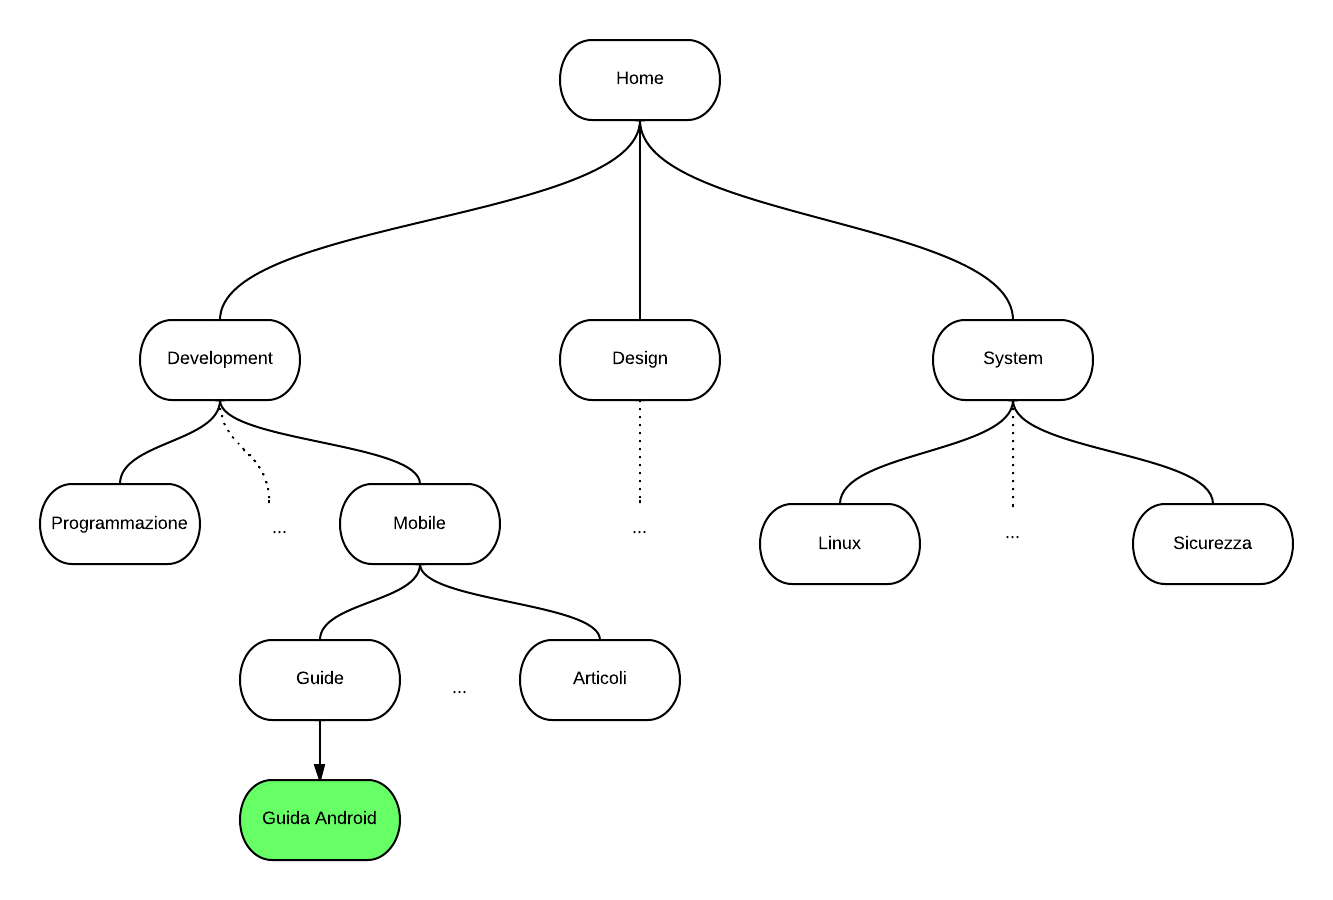
\includegraphics[width=120mm]{images/tree.png}
\caption{Struttura ad albero di html.it}
\end{figure}

In questo caso vediamo il formarsi di tre categorie principali:

\begin{itemize}

\item \textbf{Development}, contenente guide e articoli per lo sviluppo web, mobile, ecc;
\item \textbf{Design}, contiene guide e articoli per il design di applicazioni o siti web;
\item \textbf{System} che infine contiene guide e articoli per lo sviluppo e mantenimento di sistemi complessi, come ad esempio Linux.

\end{itemize}

Da queste tre categorie vi è una diramazione di sottocategorie con grana sempre più fine. Questa struttura consente all'utente di poter arrivare a ciò di cui necessita in tempi relativamente brevi.

\subsection{Sezioni}

Il sito è composto, oltre che delle sezioni riguardanti gli articoli e le guide, di altre sezioni ricche di contenuti:

\begin{itemize}

\item Una sezione \textbf{download}, dalla quale è possibile scaricare software o script generati dagli utenti;
\item Una sezione \textbf{video}, contenente una vera e propria libreria di video su un vastissimo numero di argomenti;
\item Una sezione \textbf{corsi}, in cui è possibile visualizzare una vetrina di corsi attinenti all'argomento;
\item Una sezione \textbf{forum} in cui gli utenti possono discutere di tutti gli argomenti attinenti al mondo dello sviluppo web (e non solo).

\end{itemize}

Analizzare tutte le sezioni risulterebbe un lavoro enorme e chiaramente più lungo del previsto, per cui ho deciso di analizzare solamente la sezione più navigata, ovvero quella relativa agli articoli e alle guide.		% capitolo 1
\section{Le 6 W}

Un sito web lo possiamo considerare come un negozio. Prima di entrare in un nuovo negozio l'approccio comune consiste nel guardare la \textbf{vetrina}. Questo è un punto cruciale, perchè è proprio in quel momento che decidiamo se entrare in un negozio oppure proseguire oltre. Questo avviene per il web esattamente allo stesso modo. La homepage in questo contesto è la vetrina del negozio. Come si può immaginare è impossibile o comunque poco ragionevole mostrare l'intero contenuto del negozio nella sua vetrina. Lo scopo del commerciante è quello di far sì che l'utente entri nel suo negozio, per cui è necessario attirare la sua attenzione e suscitare la sua curiosità. Le apparenze in questo campo sono molto importanti. Il proprietario del sito web deve pertanto cercare di soddisfare le cosiddette 6 W.

Supponiamo di essere un utente indefinito, non necessariamente appassionato di informatica o di sviluppo web ma comunque con un grado minimo di intelligenza e cultura. A Nel momento in cui io capito \textbf{casualmente} per la prima volta su html.it quello che vedo è rappresentato dalla figura seguente:

\begin{figure}[H]
\centering
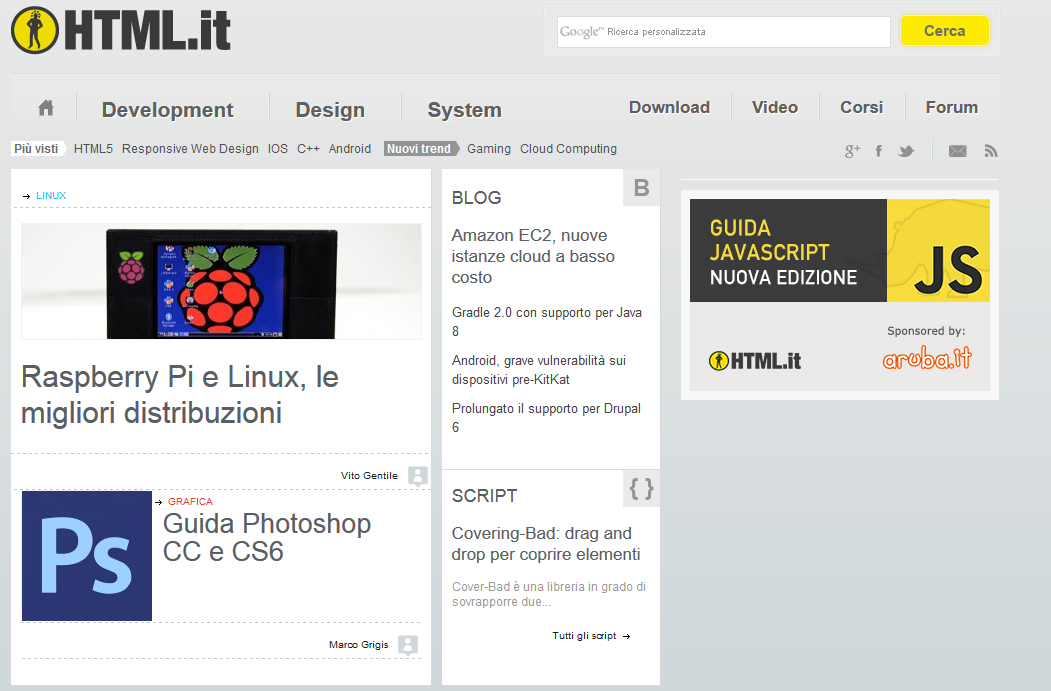
\includegraphics[width=120mm]{images/home.png}
\caption{La home page di html.it}
\end{figure}

Ho eseguito una serie di test ad una persona corrispondente al profilo indicato. Ho dato ad essa un tempo compreso tra i 10 e i 30 secondi e le ho detto di porsi le seguenti domande:

\subsection{Where?}

\begin{center}

\textit{``A che tipo di sito sono arrivato? Quale contenuto mi offre?''}

\end{center}

Il soggetto ha riconosciuto in tempi non eccessivamente lunghi che il sito si occupa di informatica e che offre la visualizzazione di articoli e guide. Ciò è stato possibile grazie alla presenza degli ultimi articoli direttamente nella home page. In questo modo è comprensibile a primo sguardo di cosa il sito tratta, per cui se il soggetto fosse stato interessato a leggere un articolo o una guida sull'argomento molto probabilmente avrebbe continuato la navigazione nel sito.

\subsection{Who?}

\begin{center}

\textit{``Chi rappresenta il sito?''}

\end{center}

Posso affermare con certezza che se il soggetto non avesse avuto la minima idea di cosa significassero termini come \textit{javascript}, \textit{raspberry} o \textit{photoshop} probabilmente ci avrebbe messo un tempo molto più alto, ragion per cui a mio modo di vedere per migliorare ques'aspetto una buona idea sarebbe quella di inserire uno slogan affianco al banner \textbf{html.it}. In questo modo a questa domanda si potrà rispondere in tempi brevissimi e inferiori ai 5 secondi, mentre allo stato attuale difficilmente si riesce a rispondere a primo impatto, ed è necessario dunque continuare la navigazione, obiettivo che è molto difficile da raggiungere.

\subsection{Why?}

\begin{center}

\textit{``Perchè mai dovrei fermarmi su questo sito? Quali benefici mi porta?''}

\end{center}

Il sito non presenta un'evidente pagina o sezione in cui viene descritto cosa esso rappresenta. Dà per scontato il fatto che il visitatore sappia esattamente dov'è arrivato e conosca precedentemente la sua fama. html.it è un sito molto rinomato, probabilmente chiunque lavora nel settore ci sarà capitato decine di volte. Ciononostante un buon sito web non può basarsi su questa supposizione, deve cercare di racchiudere nella sua cerchia il maggior numero di utenti possibili e dar loro un motivo per tornarci. In questo momento l'utente non ha un'idea molto chiara, non sa ancora se conviene soffermarsi oppure no.

Un sito web che si presenta bene ed esplicita in modo chiaro ciò che rappresenta porta all'utente un certo grado di fiducia. Come già detto prima una possibile miglioria sarebbe quella di inserire una breve descrizione nel banner e in aggiunta, a mio modo di vedere, una sezione in cui viene descritto il sito, i suoi componenti e i suoi scopi.

\subsection{What?}

\begin{center}

\textit{``Cosa offre il sito?''}

\end{center}

Supponiamo che l'utente sia stato colpito dalla home page e abbia deciso di restare per qualche minuto sul sito. A questo punto deciderà dunque di guardarsi intorno, scrollerà probabilmente verticalmente verso il basso e ciò che vedrà sarà la Figura ~\ref{fig:f3}.

\begin{figure}[H]
\centering
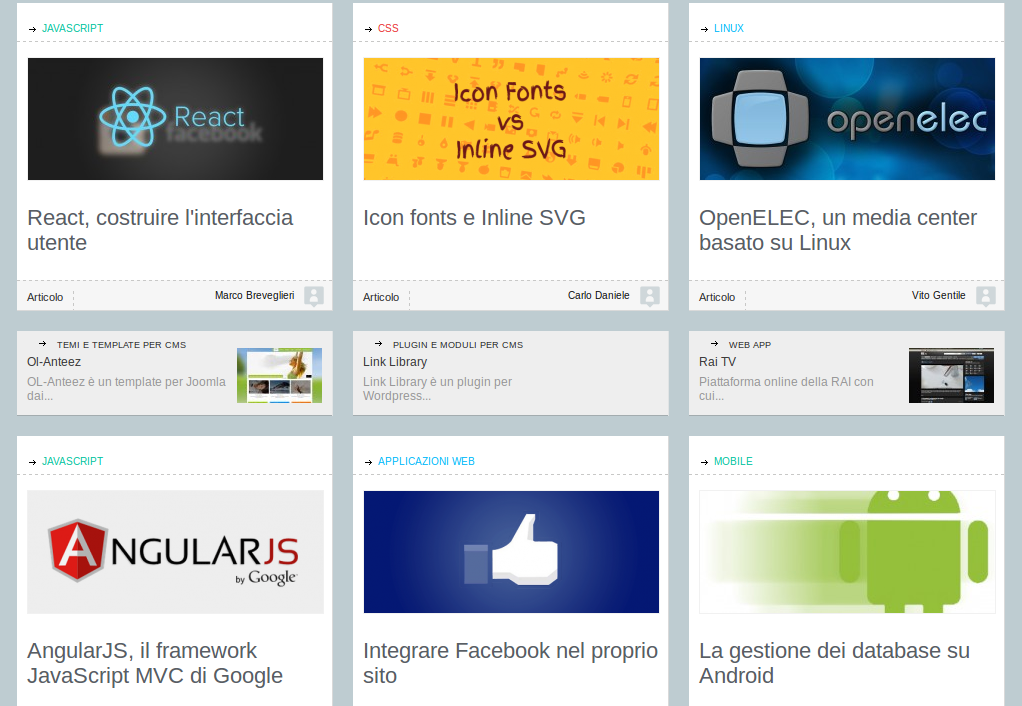
\includegraphics[width=120mm]{images/screen1.png}
\caption{La home page con uno scroll verso il basso}
\label{fig:f3}
\end{figure}

Come possiamo vedere troviamo tutta una serie di guide e articoli su diversi argomenti, il tutto disposto con visualizzazione a griglia. Questo è chiaramente un punto a favore, la visualizzazione a griglia è risultata (ed è tuttora) molto popolare negli ultimi anni, basti pensare alle interfacce di sistemi operativi come Android o iOS per gli smartphone o l'interfaccia Metro di Windows 8. L'avere un'interfaccia di questo tipo evita l'utente di scrollare troppo verso il basso per accedere ai contenuti e quindi lo stress è notevolmente diminuito. Ciascuno di questi ``mattoncini'' è cliccabile e il link rimanda alla relativa guida o articolo. La home page risponde quindi molto bene a questa domanda.

Una cosa molto fastidiosa però è rappresentata dalla figura seguente:

\begin{figure}[H]
\centering

\includegraphics[width=50mm]{images/detail1.png}
\caption{Possibile link che non è un link}
\end{figure}

Ho segnato in rosso un difetto piuttosto rilevante. Chiunque vedendo l'articolo e la sua categoria si aspetta di cliccare sulla categoria ed essere rimandati ad una pagina contenente la lista degli ultimi articoli riguardanti quella categoria. Questo però non avviene e il possibile link è in realtà del semplice testo. Questo crea sicuramente frustrazione all'utente e fa chiaramente perdere i punti che il sito si era guadagnato con la visualizzazione a griglia.

\subsection{When?}

\begin{center}

\textit{``Quali sono le ultime novità? Quando è stato manutenuto per l'ultima volta?''}

\end{center}

Il sito risponde molto bene a questa domanda. Nella home page sono presenti gli ultimi articoli inseriti e ogni giorno è possibile scoprire i contenuti nuovi. Questo è importantissimo, perchè non c'è cosa peggiore di dare all'utente la sensazione di staticità. Se si vuol far sì che l'utente sia invogliato a tornare, bisogna fargli credere che quando tornerà per la seconda o terza o n-esima volta troverà sempre contenuti aggiornati e nuovi articoli o guide interessanti. Dare evidenza di manutenibilità di un sito web produce molta affidabilità e dà all'utente una fiducia non indifferente.



\subsection{How?}

\begin{center}

\textit{``Come faccio ad arrivare alle sezioni principali?''}

\end{center}

In questo caso il sito presenta un aspetto buono e uno non buono. Il fatto positivo è che la navigazione è tutto sommato ben strutturata. Come sottolineato nel precedente capitolo le guide e gli articoli si suddividono in tre categorie principali:

\begin{enumerate}

\item Development;
\item Design;
\item System.

\end{enumerate}

Il menu di navigazione evidenzia questi tre macro livelli e permette la navigazione al livello inferiore tramite un menu a tendina, come mostrato nella due figure seguenti:

\begin{figure}[H]
\centering

\includegraphics[width=120mm]{images/menu.png}
\caption{Menu di navigazione a tendina chiusa}
\end{figure}

\begin{figure}[H]
\centering
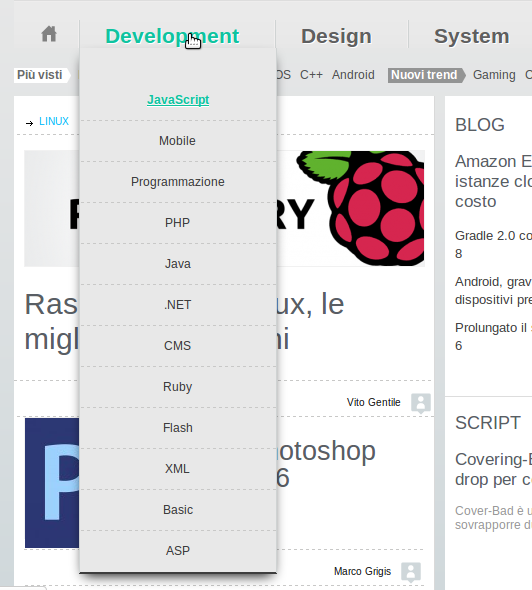
\includegraphics[width=80mm]{images/menu1.png}
\caption{Menu a di navigazione a tendina aperta}
\end{figure}

Il menu a tendina è facilmente navigabile ed è intuitivo, inoltre fa sì che il menu occupi poco spazio nell'intera pagina, dando più peso dunque al contenuto. Tramite questo menu l'utente può destreggiarsi all'interno del sito e raggiungere le sezioni a cui è interessato. Inoltre sotto al menu sono presenti i link alle guide e agli articoli più visitati, cosa sicuramente molto utile.

L'aspetto negativo è che da un lato il menu è poco visibile e non risalta all'occhio in modo immediato, mentre dall'altro nel momento in cui io scrollo verticalmente verso il basso esso sparisce, costringendomi a scrollare nuovamente verticalmente verso l'alto per tornare ad esso. Ora, questa è decisamente una mia opinione, ma credo che se si utilizzasse un menu fisso che risulta sempre visibile lungo tutta la navigazione si guadagnerebbe qualche punto in usabilità. Chiaramente può dare fastidio ed essere visivamente ingombrante. In tal caso una soluzione sarebbe ridurre lo spessore e renderlo simile alla barra di navigazione di facebook. Questa però è solamente la mia opinione.

			% capitolo 2
\section{Il contenuto}		% capitolo 3
\section{La pubblicità}

Questo aspetto è sicuramente importantissimo per la navigazione e l'usabilità. È perfettamente comprensibile che un sito web tragga dei profitti dal proprio lavoro, ed in questo caso essi provengono in primis dalla pubblicità. C'è però modo e modo di gestirla. Gli utenti nella quasi totalità dei casi odiano la pubblicità e chiaramente vorrebbero farne a meno. Esistono plugin per i diversi browser che bloccano le pubblicità ma non cancellano definitivamente il problema.

\subsection{Pubblicità sul layout}

Ora ho disattivato il mio adblocker su firefox e il risultato sono queste aggiunte:

\begin{figure}[H]
\centering

\includegraphics[width=100mm]{images/adv1.png}
\caption{Pubblicità sotto il menu di navigazione}
\end{figure}

\begin{figure}[H]
\centering

\includegraphics[width=100mm]{images/adv2.png}
\caption{Pubblicità in mezzo al menu}
\end{figure}

\begin{figure}[H]
\centering
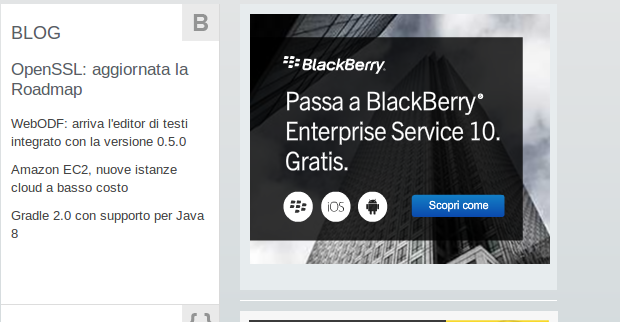
\includegraphics[width=100mm]{images/adv3.png}
\caption{Pubblicità sulla barra laterale}
\end{figure}

Niente di così grave per il momento, in ogni caso più un meno lungo l'intera pagina compaiono pubblicità di ogni tipo, non necessariamente legate al mondo dell'informatica. Questo ancora non è fastidioso ed è sopportabile dall'utente. Una cosa leggermente più vistosa è quando la pubblcità compare sullo sfondo del sito, come in questo caso:

\begin{figure}[H]
\centering

\includegraphics[width=120mm]{images/adv6.png}
\caption{Pubblicità sullo sfondo}
\end{figure}

Come si può notare distoglie chiaramente l'attenzione e provoca frustrazione all'utente.

\subsection{Pop-up}

Una cosa peggiore arriva nel momento in cui cerco di accedere ad un'articolo o una guida. Il risultato è il seguente:

\begin{figure}[H]
\centering
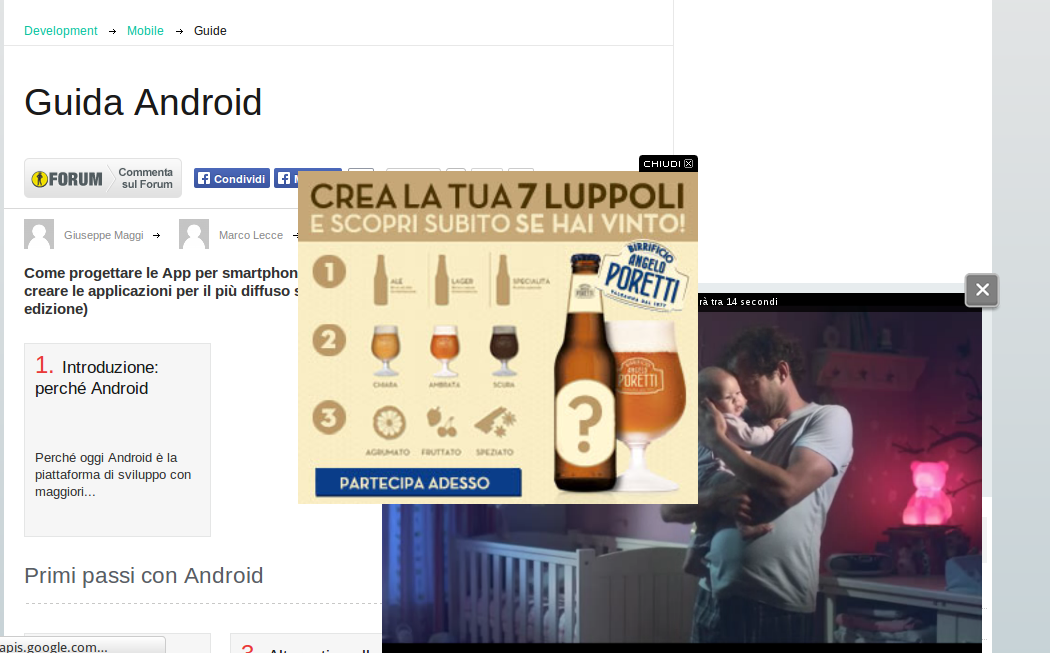
\includegraphics[width=120mm]{images/adv4.png}
\caption{Pop-up all'apertura di un'articolo}
\end{figure}

Come si può notare è apparso un fastidiosissimo pop-up che blocca completamente la lettura e costringe l'utente a chiuderlo. Se l'utente sbaglia a cliccare il pulsante di chiusura rischia chiaramente di essere reindirizzato ad un altro sito. Questa è decisamente una mazzata per l'usabilità, fa passare la voglia a qualunque utente di rimanere nel sito.

\subsection{Video}

Il peggio purtroppo non è ancora arrivato. Se noi abilmente chiudiamo il pop-up sotto possiamo ammirare un bellissimo video (non richiesto) che invade il contenuto della pagina e che parte tranquillamente in automatico anche con il volume.


\begin{figure}[H]
\centering
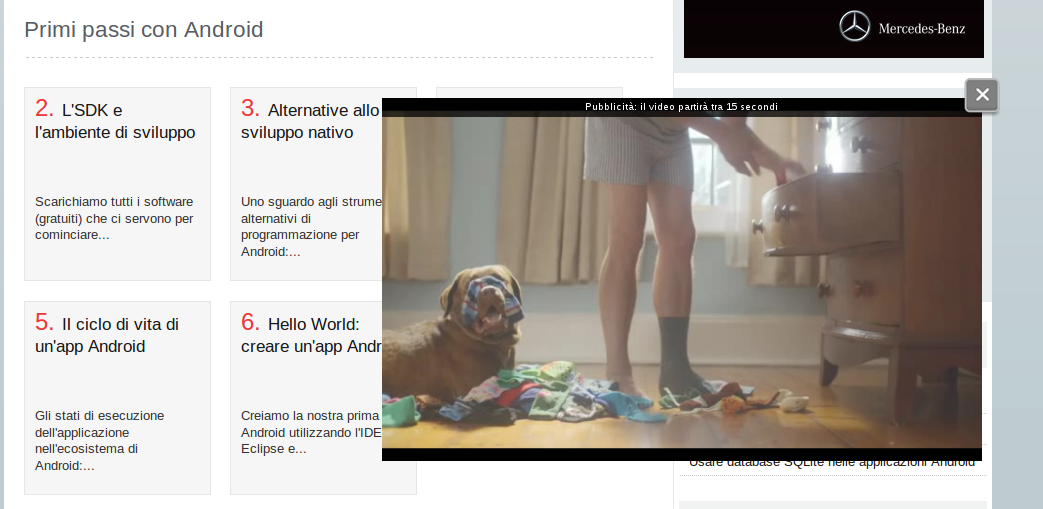
\includegraphics[width=120mm]{images/adv5.png}
\caption{Video di pubblicità invadente}
\end{figure}

Questa è una combo micidiale per l'usabilità, è probabilemente ancora peggio della finestra pop-up precedente. Noterete inoltre come sia incredibilmente ostico mettere il video in pausa.
\linebreak
\linebreak
Tutto questo avviene lungo l'intera navigazione e per ciascuna lezione c'è il video di pubblicità che per la nostra felicità compare ogni volta e disturba la nostra lettura. Questo comporta uno stress notevole da parte dell'utente e una sua diffidenza. Personalmente io evito tutto questo con un adblocker ma un utente normale in questa situazione si ritroverebbe sommerso da pubblcità invadente e fuori contesto senza suo malgrado poter porre rimedio.
\linebreak
\linebreak
In conclusione, la pubblicità è lecita e comprensibile ma questo sito la gestisce in modo pessimo ammazzando letteralmente l'usabilità. Questo aspetto fa precipitare l'intero giudizio del sito, fin qui tutto sommato buono.
	% capitolo 4
\section{La ricerca}

html.it è un autentico portale più che un sito web. Consiste di decine, forse centinaia di articoli e guide, si sviluppa su diversi rami e raccoglie un'infinità di informazione. Quando si ha a che fare con siti web di questa portata è essenziale dotare il medesimo di un sistema di \textbf{ricerca interna} che sia il più eccellente possibile e soprattutto che sia simile al modo in cui l'utente è solitamente abituato ad effettuare la ricerca.

html.it utilizza un tool di google per effettuare ricerche interne al sito. Questa è una soluzione veloce, a costo zero ed efficace in quanto utilizza il motore di ricerca google che è indubbiamente il più utilizzato nel web. La barra di ricerca è molto ben visibile e può contenere un buon numero di caratteri (>30). Proviamo ad effettuare una ricerca e vediamo i risultati ottenuti. Cerchiamo ad esempio il termine ``usabilità'':

\begin{figure}[H]
\centering
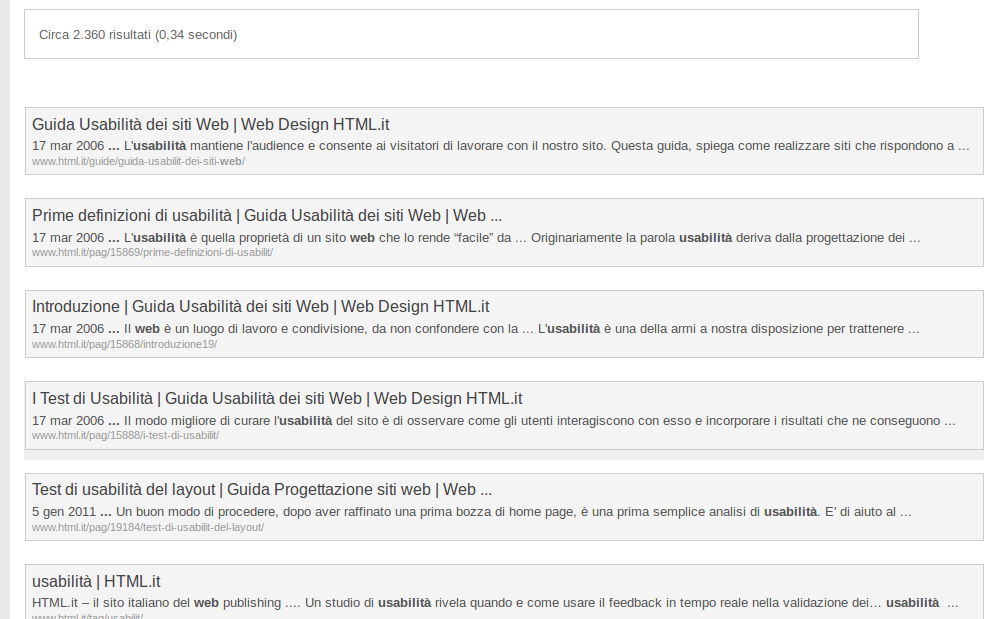
\includegraphics[width=120mm]{images/search.png}
\caption{I risultati di una ricerca}
\end{figure}

Come possiamo vedere la ricerca produce tutti risultati interni al sito in modo paginato visualizzandoli a lista e riesce a rispondere in modo efficiente alla nostra richiesta. Questo approccio è ottimo, purchè progettato per funzionare su bassa scala. Se infatti l'utente riusa la ricerca interna fatta precedentemente all'esterno significa che il motore di ricerca non gli ha fornito l'informazione cercata e quindi la ricerca fatta allo stesso modo produrrà il medesimo risultato. Inoltre i motori di ricerca troncano il 50\% delle indicizzazioni, quindi verrà fatto anche in locale, con perdita della metà delle informazione.

In conclusione la soluzione adottata è buona, fornisce quanto richiesto ma non è la soluzione ottima. L'idea migliore sarebbe quella di sviluppare un motore di ricerca interno progettato dagli sviluppatori del sito in modo che effettui ricerche in base alla struttura del sito. Ciò chiaramente comporta un costo in termini di tempi e risorse da impiegare per la progettazione e la codifica. Cionondimeno sarebbe sicuramente una buona feature da sviluppare in futuro.


		% capitolo 5
\section{Valutazioni e considerazioni finali}	% capitolo 6

%\appendix

%\input{glossario}


\end{document}
